\paragraph{}This chapter will explain the methodology and requirements for the \ac{SLAM} tuning module, developed for \ac{RUSTLE}. For each implemented tuning technique, a high level overview of its architecture is provided. Test settings, including test algorithms and dataset choices, are also justified.

\begin{figure}[h]
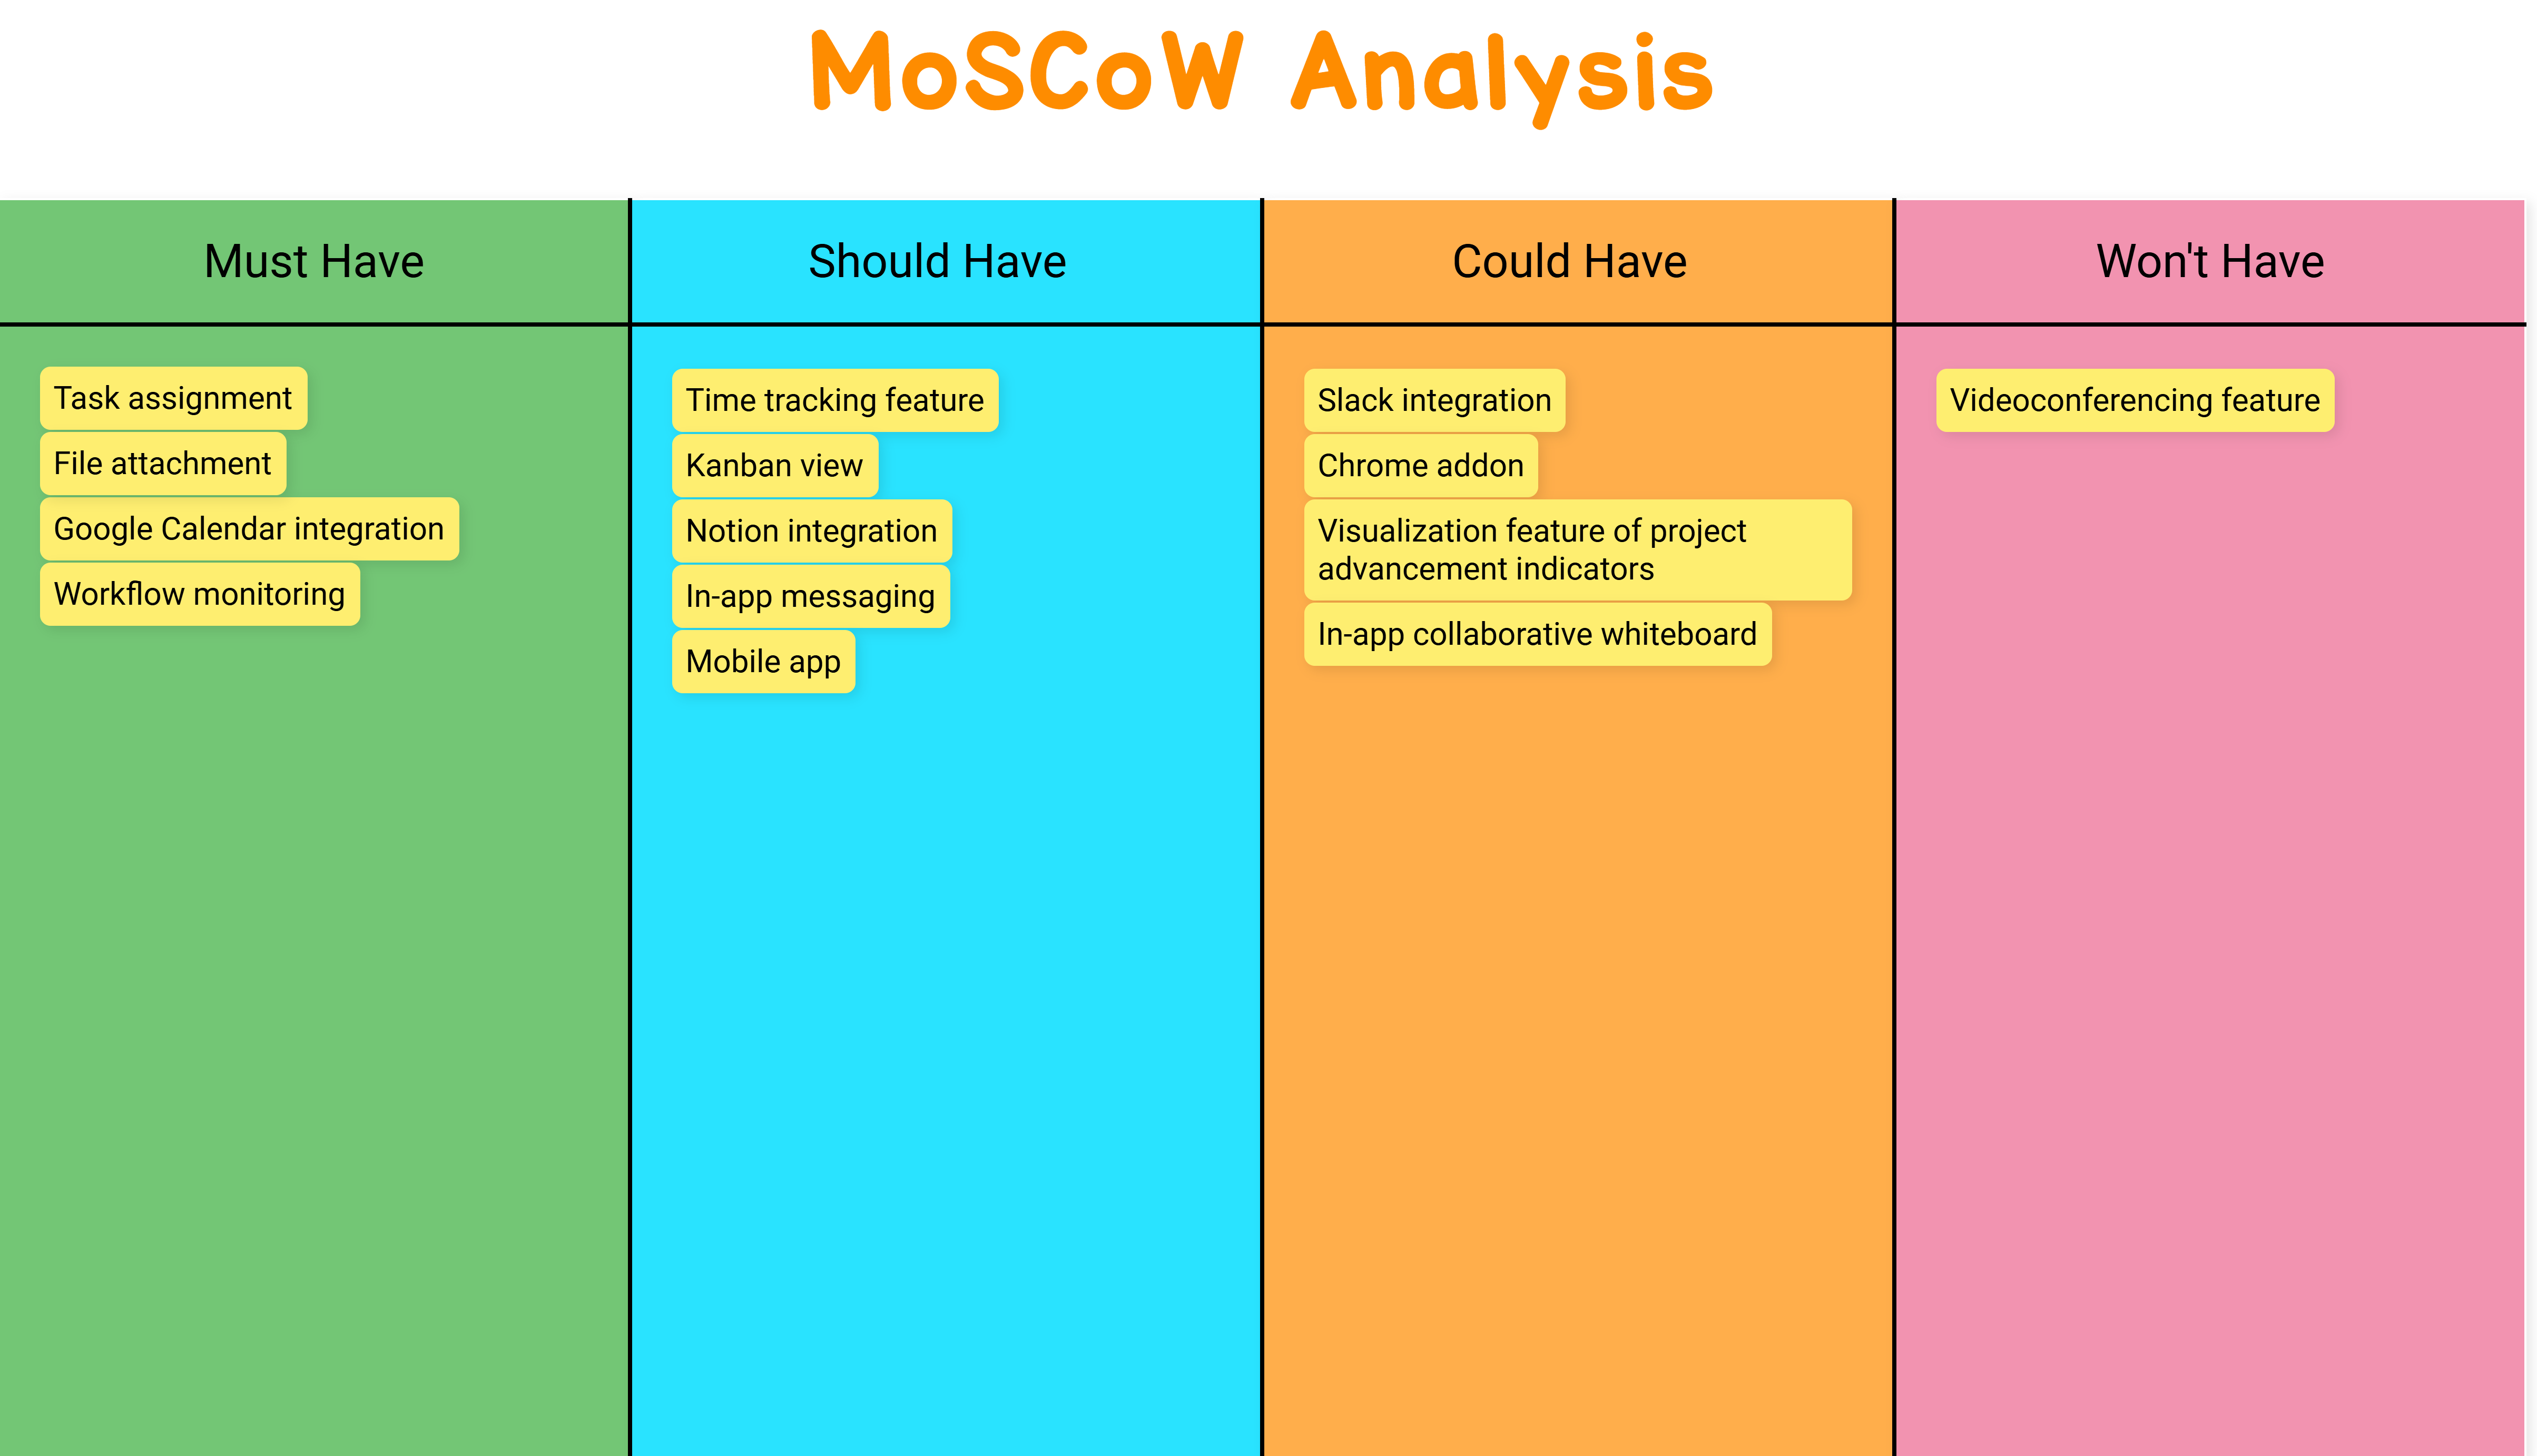
\includegraphics[width=0.85\linewidth]{images/moscow.png}
\end{figure}

\section{\ac{RUSTLE}}

\paragraph{}\ac{RUSTLE} is a command line application, written in Rust, which is designed to simplify the evaluation of SLAM algorithms in mobile robotics.
Its main objective is to provide a simple, stream-lined and reproducible way to run and compare SLAM algorithms. It tracks not only trajectory accuracy(APE or RPE), but also runtime, CPU load and memory usage, offering a more complete assessment of the algorithm's performance.

\paragraph{}At its core, RUSTLE takes three main inputs: a dataset in rosbag format, the SLAM algorithm's parameters in yaml format, and the algorithms themselves as docker images. The reason for using Docker is for reliably reproducing the algorithms across many different platforms and environments.
During execution, the odometry data is streamed into the database(Surrealdb), which, after conclusion, is used to calculate trajectory errors such as the APE and the RPE, using EVO.

\paragraph{}Algorithm executions are run as tests. Each test's configuration is passes as an YAML file, and contains: its name, number of workers, number of iterations, list of algorithms, dataset on which to execute these algorithms and the test type. Additionally, some additional fields might be required, depending on the type of test one wants to execute.

\paragraph{}As for language choice, Rust was chosen mostly due to simplicity of development and the ease with which one can write highly performant code. Other languages, such as c++ and python, also have libraries for working with Docker and ROS, as well as libraries for database hosting. The difference with Rust in this regard is that to use these libraries it is only needed to include them as dependencies, and use them in the codebase, as the download, compilation and linking of these libraries is all automatically handled by Rust's build tool, cargo. As for performance, Rust is known for its compile-time enforced memory safety(at the cost of some control over memory), as well as built in type system guarantees, which prevent common multithreaded issues like data races.

\section{Development}
\paragraph{}Development follows an incremental approach, focusing on small incremental features, well thought and tested. Each big feature, such as random search tuning, is divided into smaller "implementable" sub-features. The reason for this is to make it easier to reason about how to implement the feature, as well as, during development, to make it easier to test each sub-feature.

\section{Functional requirements}

\paragraph{}The system must allow users to define all relevant settings for the tuning process using a YAML configuration file. This configuration file will serve as the main interface for specifying the tuning method, SLAM algorithm, and dataset to be used. In addition, it will enable the user to indicate which parameters are to be optimized, with one or more values per parameter. Additionaly, the code must ensure type safety, meaning, for example, that a parameter which is supposed to be a String cannot have a u64 passed as a value.

\paragraph{}For grid and random search tuning methods, the configuration file must support flexible representations of parameter values. Each tunable parameter can be defined as a single value, representing a fixed setting, or as an array containing multiple candidate values to be tested. For numerical parameters(integers and floats), a third specification pattern must be supported: a linearly spaced vector. This vector will be described by a three-element array in the form \textbf{[start, step, number\_of\_elements]}, which the system will interpret to automatically generate a sequence of values. This feature will simplify the definition of evenly spaced search spaces for numerical parameters and ensures consistency across different tuning runs. It also makes it significantly less cumbersome to define large sequences of values.

\paragraph{}Every tuning algorithm has, besides the parameter space, some method specific hyperparameters that control its behavior, such as the budget(grid search) or the cooling factor(SA). Each of these parameters must have a default value, so the user doesn't need to fine tune the tuning algorithm's behavior. As for the budget \textbf{B}, a common hyperparameter used in tuning algorithms, it must be either time based, or iterations based(maximum number of iterations to run).

\paragraph{}For easier development and integration with the overall code structure of RUSTLE, the tuning of an algorithm's hyperparameters is treated as a test. Each configuration is run as a \textbf{simple test}, already defined in the code, changing hyperparameters between iterations. This methodology will allow for greater re-usage of already written code, saving on development time.

\paragraph{}When running a tuning test, each configuration and its metrics(results) must be stored for later processing. The tuning method's hyperparameters must be stored as well, mostly for benchmarking purposes.

\paragraph{}For benchmarking different tuning algorithms, there must be a command as simple as \textbf{tune benchmark -algo xxxxx -dataset xxxxx}, which runs a few preselected tuning algorithms, and displays a few performance metrics.

\paragraph{}Whenever possible, configurations should be run concurrently.

\paragraph{}The code written should be future proof, allowing for easier future integrations of more tuning methods into the software.


%\begin{itemize}
	%\item allow the user to specify which tuning method, algorithm and dataset, and also the parameters to optimize using a yaml configuration file.
	%\item For grid and random search, for any tuned parameters in the configuration file, the general pattern should be either a single value or an array of various values. For numerical parameters(integers or real numbers), a third option must be available: a linearly spaced vector, and that vector is specified through a 3 element array whose elements are [start, step, number\_of\_elements], allowing for the specification of arrays of  n values, without the cumbersomeness of manually specifying all the values.
	%\item Other settings, such as the budget or the cooling factor in the simulated annealing method, should have default values
	%\item a budget parameter(B) should be either a maximum number of configurations to run or maximum alloted time. These should be represented by the keys \textbf{max\_iter} and \textbf{max\_time} in the configuration file.
	%\item tuning a SLAM algorithm's parameters is classified as a test, for easier integration in the existing RUSTLE's architecture.
	%\item when running a tuning test, all tested parameter combinations should have their respective metrics stored together, for later processing
	%\item when running a tuning test, all tuning settings should be stored as well, for later processing and examination
	%\item for overall testing and comparison of different tuning strategies, there should be a command to run a set of tuning algorithms and produce appropriate metrics which later could be displayed as a table or graph.
	%\item The tuning module should run different configurations concurrently, when possible.
%\end{itemize}

\section{Non Functional requirements}

%\begin{itemize}
%	\item The tuning module should be future proof, allowing for the easy addition of other tuning algorithms into the software.
%	\item 
%\end{itemize}

\section{Testing}

\subsection{Metrics}

\subsection{Algorithms}

\subsection{Datasets}